

\section{AnisoCADO%
  \label{anisocado}%
}

A package for analytically generating SCAO PSFs primarily for the ELT

Documentation: \url{https://anisocado.readthedocs.io/}

Code Base: \url{https://github.com/astronomyk/AnisoCADO}

Continuous integration : \url{https://travis-ci.org/github/astronomyk/AnisoCADO}

Author: Kieran Leschinski


\subsection{Introduction%
  \label{introduction}%
}

\begin{itemize}
\item 
\begin{description}
\item[{Why AnisoCADO exists}] \leavevmode 
\begin{itemize}
\item Quickly create SCAO PSFs
\end{itemize}

\end{description}

\item 
\begin{description}
\item[{Limiting assumptions}] \leavevmode 
\begin{itemize}
\item Long exposure PSFs (> D\_M1 / v\_wind)

\item No coherence between time steps
\end{itemize}

\end{description}
\end{itemize}


\subsection{Examples%
  \label{examples}%
}

\begin{itemize}
\item Basic use case

\item Off-axis
\end{itemize}

\phantomsection\label{code-anisocado-example}
\begin{DUclass}{code}
\begin{DUclass}{execute}
\begin{quote}
\begin{alltt}
from anisocado import AnalyticalScaoPsf

psf = AnalyticalScaoPsf(N=64, wavelength=2.15)  # um
on_axis = psf.psf_on_axis
off_axis = psf.shift_off_axis(15, -5)   # arcsec
\end{alltt}
\end{quote}
\end{DUclass}
\end{DUclass}

% action: plot
% name: anisocado_basic_example
% ---
% plt.figure(figsize=(10,5))
% plt.subplot(121)
% plt.imshow(on_axis, norm=LogNorm())
% plt.subplot(122)
% plt.imshow(off_axis, norm=LogNorm())

\begin{figure}[H]
\noindent\makebox[\linewidth][c]{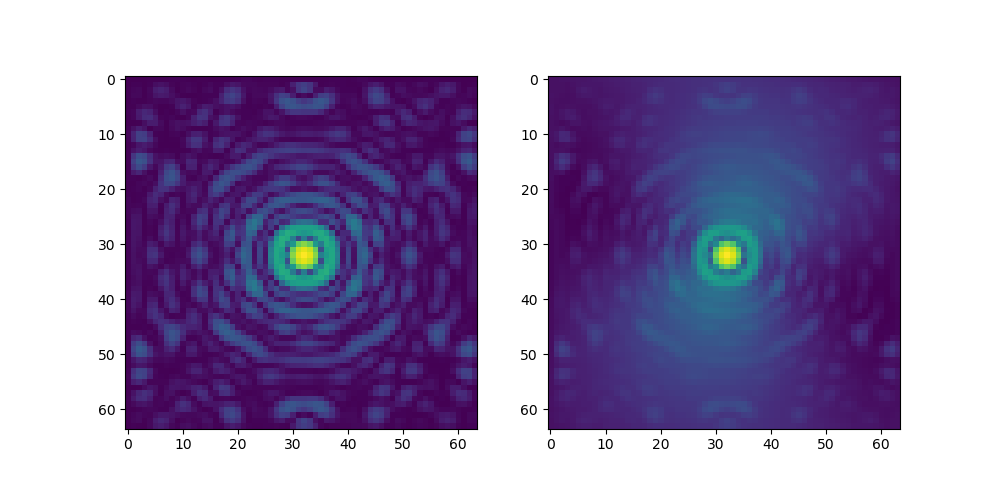
\includegraphics[scale=0.500000]{images/anisocado_basic_example.png}}\phantomsection\label{fig-anisocado-basic-example}

\caption{Left: the on-axis K-band (2.15\$mu\$m) SCAO PSF for standrard atmospheric conditions.
Right: the K-band SCAO-PSF at the position (15, -5) arcseconds from the natural guide star.}
\end{figure}


\subsection{Functionality%
  \label{functionality}%
}

\begin{itemize}
\item How AnisoCADO creates the SCAO PSFs

\item Long / Short exposure PSFs

\item Off axis

\item Wavelength dependence
\end{itemize}
